\documentclass[border=10pt]{standalone}
\usepackage[svgnames]{xcolor}
\usepackage{amsmath}
\usepackage{pgfplots}
\pgfplotsset{compat=newest}
\usepackage[sfdefault]{FiraSans}
\usepackage{FiraMono}
\renewcommand*\familydefault{\sfdefault}
\begin{document}
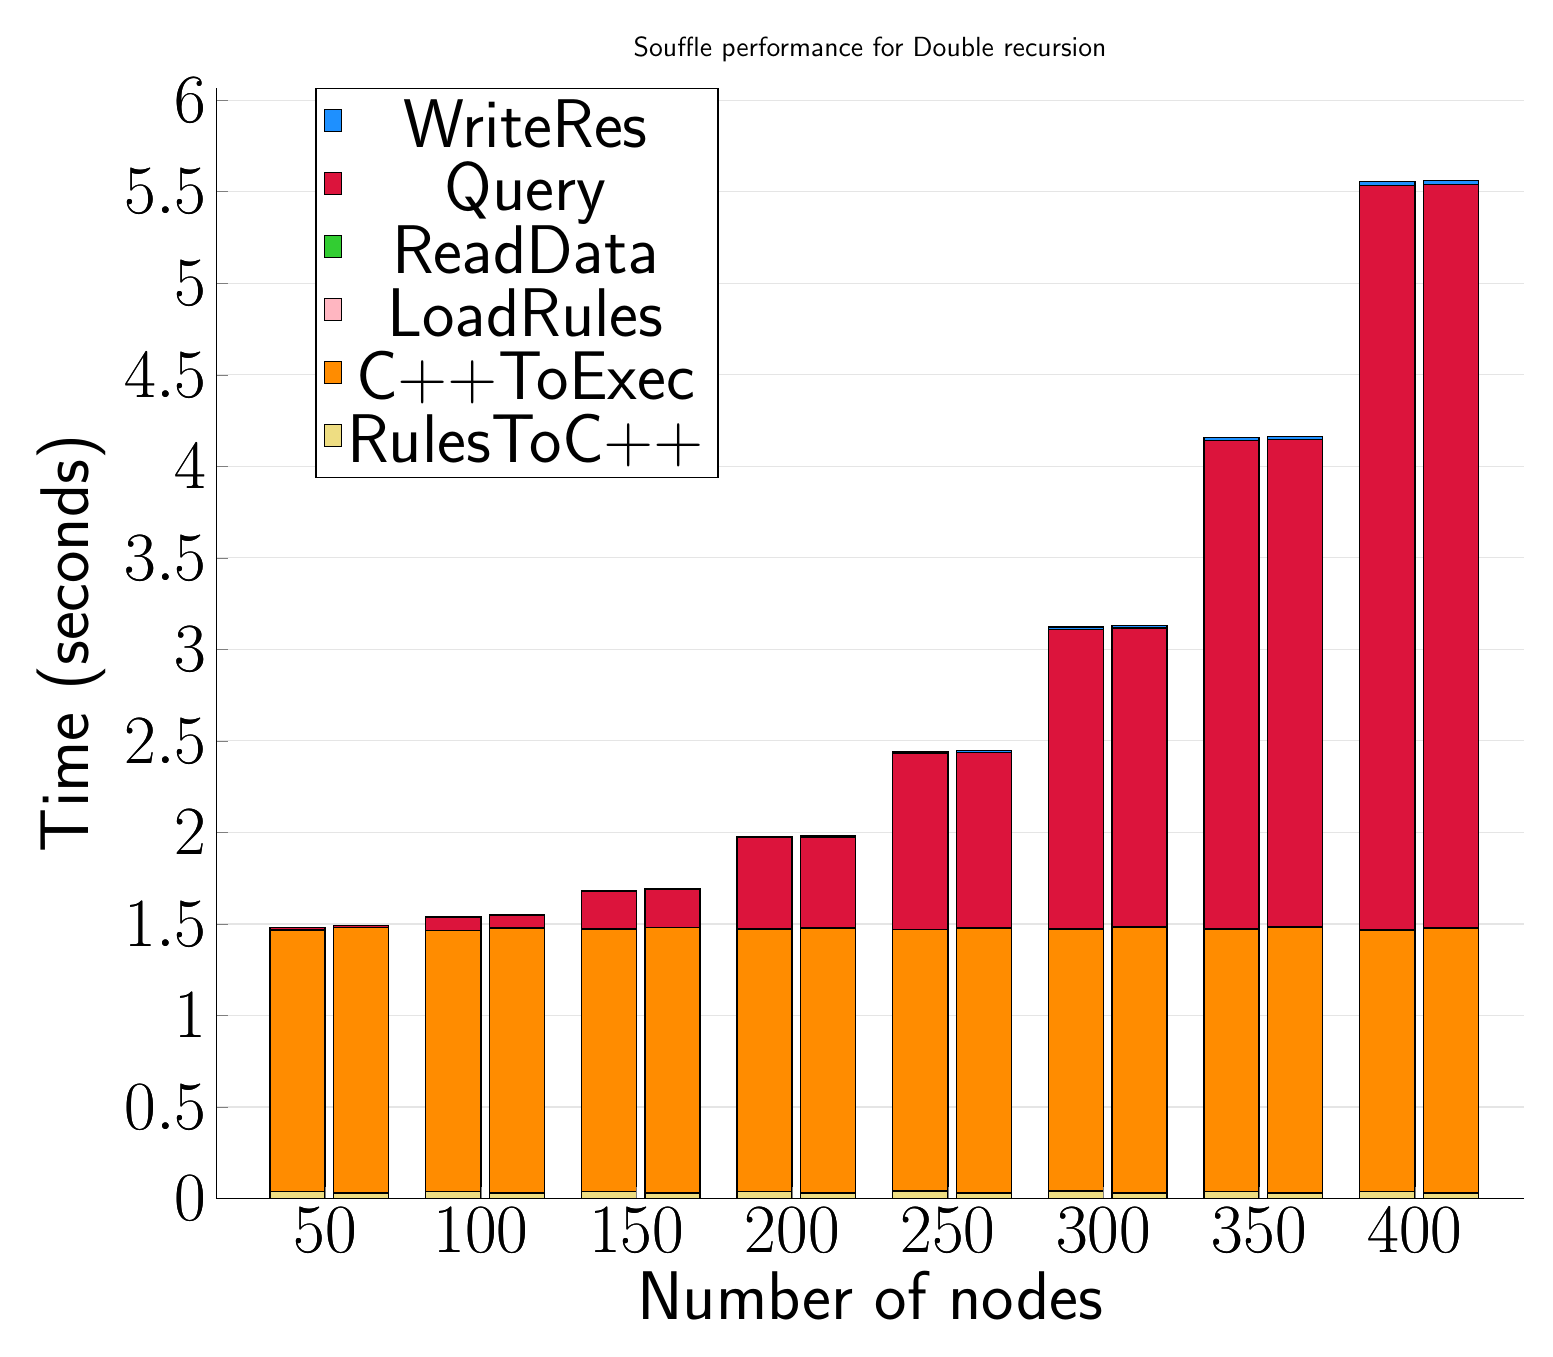
\begin{tikzpicture}
\begin{axis}[
   ybar stacked,
   title={Souffle performance for Double recursion},
   bar shift=-10pt,
   width=1.5\textwidth,
   bar width=0.7cm,
   ymajorgrids, tick align=inside,
   major grid style={draw=gray!20},
   xtick=data,
   ymin=0, ymax=6.067577,
   axis x line*=bottom,
   axis y line*=left,
   enlarge x limits=0.1,
   legend style={
       at={(0.23, 1)},
       anchor=north,
       legend columns=1,
       font=\Huge,
   },
   ylabel={Time (seconds)},
   xlabel={Number of nodes},
   label style={font=\Huge},
   tick label style={font=\Huge},
]
\addlegendimage{fill=DodgerBlue, draw=black, line width=0.2pt}
\addlegendentry{WriteRes}
\addlegendimage{fill=Crimson, draw=black, line width=0.2pt}
\addlegendentry{Query}
\addlegendimage{fill=LimeGreen, draw=black, line width=0.2pt}
\addlegendentry{ReadData}
\addlegendimage{fill=LightPink, draw=black, line width=0.2pt}
\addlegendentry{LoadRules}
\addlegendimage{fill=DarkOrange, draw=black, line width=0.2pt}
\addlegendentry{C++ToExec}
\addlegendimage{fill=LightGoldenrod, draw=black, line width=0.2pt}
\addlegendentry{RulesToC++}
\addplot +[fill=LightGoldenrod, draw=black, line width=0.5pt] coordinates {
    (50, 0.04000003337860107)
    (100, 0.039999985694885255)
    (150, 0.039999985694885255)
    (200, 0.039999985694885255)
    (250, 0.04100000858306885)
    (300, 0.040999984741210936)
    (350, 0.039999985694885255)
    (400, 0.039999985694885255)
};
\addplot +[fill=DarkOrange, draw=black, line width=0.5pt] coordinates {
    (50, 1.4269999980926513)
    (100, 1.4250000238418579)
    (150, 1.431000018119812)
    (200, 1.431999969482422)
    (250, 1.4289999961853028)
    (300, 1.431000018119812)
    (350, 1.4319999933242797)
    (400, 1.425)
};
\addplot +[fill=LightPink, draw=black, line width=0.5pt] coordinates {
    (50, 8.442940000000002e-05)
    (100, 0.0001263294)
    (150, 0.0001095501)
    (200, 0.00011414160000000002)
    (250, 9.805e-05)
    (300, 9.81043e-05)
    (350, 8.8675e-05)
    (400, 9.652920000000001e-05)
};
\addplot +[fill=LimeGreen, draw=black, line width=0.5pt] coordinates {
    (50, 0.0003154666)
    (100, 0.00047821260000000004)
    (150, 0.0005573250999999999)
    (200, 0.0006621126)
    (250, 0.0007669874)
    (300, 0.0008501874)
    (350, 0.0010094918999999998)
    (400, 0.0010485414)
};
\addplot +[fill=Crimson, draw=black, line width=0.5pt] coordinates {
    (50, 0.011798501999999999)
    (100, 0.07249712)
    (150, 0.20776840000000002)
    (200, 0.49803189999999997)
    (250, 0.9597423)
    (300, 1.635692)
    (350, 2.6678699999999997)
    (400, 4.067577)
};
\addplot +[fill=DodgerBlue, draw=black, line width=0.5pt] coordinates {
    (50, 0.0006745626000000001)
    (100, 0.001541468)
    (150, 0.0034076370000000003)
    (200, 0.00604128)
    (250, 0.008885818)
    (300, 0.01333085)
    (350, 0.01751537)
    (400, 0.02280457)
};
\end{axis}
\begin{axis}[
   ybar stacked,
   bar shift=13pt,
   width=1.5\textwidth,
   bar width=0.7cm,
   ymajorgrids, tick align=inside,
   major grid style={draw=none},
   xtick=data,
   ymin=0, ymax=6.067577,
   axis x line*=none,
   axis y line*=none,
   enlarge x limits=0.1,
   label style={font=\Huge},
   tick label style={font=\Huge},
]
\addplot +[fill=LightGoldenrod, draw=black, line width=0.5pt] coordinates {
    (50, 0.030000000000000006)
    (100, 0.031000000000000007)
    (150, 0.030000000000000006)
    (200, 0.030000000000000006)
    (250, 0.030000000000000006)
    (300, 0.030000000000000006)
    (350, 0.030000000000000006)
    (400, 0.030000000000000006)
};
\addplot +[fill=DarkOrange, draw=black, line width=0.5pt] coordinates {
    (50, 1.4499999999999997)
    (100, 1.4459999999999997)
    (150, 1.4499999999999997)
    (200, 1.4469999999999998)
    (250, 1.4489999999999996)
    (300, 1.4529999999999998)
    (350, 1.452)
    (400, 1.4479999999999997)
};
\addplot +[fill=LightPink, draw=black, line width=0.5pt] coordinates {
    (50, 8.39e-05)
    (100, 0.0001254)
    (150, 0.0001088)
    (200, 0.00011290000000000002)
    (250, 9.71e-05)
    (300, 9.709999999999999e-05)
    (350, 8.81e-05)
    (400, 9.6e-05)
};
\addplot +[fill=LimeGreen, draw=black, line width=0.5pt] coordinates {
    (50, 0.000315)
    (100, 0.0004771000000000001)
    (150, 0.0005564000000000001)
    (200, 0.0006613)
    (250, 0.0007648)
    (300, 0.0008494999999999999)
    (350, 0.0010083)
    (400, 0.0010474)
};
\addplot +[fill=Crimson, draw=black, line width=0.5pt] coordinates {
    (50, 0.011792299999999999)
    (100, 0.07234399999999999)
    (150, 0.20729199999999998)
    (200, 0.49711340000000004)
    (250, 0.9581066)
    (300, 1.632516)
    (350, 2.6630190000000002)
    (400, 4.059334)
};
\addplot +[fill=DodgerBlue, draw=black, line width=0.5pt] coordinates {
    (50, 0.0006728000000000001)
    (100, 0.0015403)
    (150, 0.0034043)
    (200, 0.005867700000000001)
    (250, 0.008877800000000002)
    (300, 0.0127716)
    (350, 0.0173661)
    (400, 0.0226163)
};
\end{axis}
\end{tikzpicture}

\end{document}
